\chapter{Stato dell'arte}

\section{Studi sull’engagement all’interno degli ambienti di studio}
Gli studi ritrovati che effettuano quest’analisi o trattano un argomento simile o tangente sono:
\subsection{Recognizing Cognitive Emotions in E-Learning Environment [1]:}
In questo studio gli stati di d’animo che vengono classificati dal loro sistema sono i seguenti:
\begin{itemize}
    \item Entusiasmo,
    \item Interesse,
    \item Sorpresa,
    \item Noia,
    \item Perplessità,
    \item Frustrazione,
    \item Neutrale
\end{itemize}

Viene riportato che gli stati d’animo positivi (entusiasmo, interesse e sorpresa) sono spesso associati al raggiungimento del “flow state” da parte dello studente.

Più il singolo soggetto mantiene costante un mood positivo, tanto più permarrà in questo flow state, con esito un apprendimento più veloce ed efficace.

Il raggiungimento di questo mood è stato inoltre connesso alla capacità dei singoli studenti di percepirsi come autosufficienti nel corso dell’attività di studio.

Questa percezione di sé stessi deriva dall’attitudine dello studente nel riuscire ad essere in controllo della sua personale situazione di studio, rispecchiandosi nella sua abilità di:
\begin{itemize}
    \item pianificare,
    \item controllare,
    \item dirigere
\end{itemize}
l’attività di apprendimento.

È quindi necessario che gli studenti maturino una certa dimestichezza nello studio, e che vengano dunque supportati in vista dell’approccio ai problemi che vengono da loro riconosciuti in quanto difficili.

Naturalmente un sistema che permette di “leggere” con precisione lo stato d’animo di uno studente/studentessa o persino di un’intera classe, e quindi capire se questi si trovino nello stato di flow che possa permettere una migliore performance, è uno strumento utile per qualsiasi insegnante.

Un esempio circoscritto all’ambiente di lavoro potrebbe invece essere un’analisi del lavoratore nello svolgimento di un task e la possibilità, da parte di un capo progetto o di un tutor, di poter intervenire esclusivamente nel momento in cui il suo subordinato sta riscontrando dei problemi; in tal modo è permessa al dipendente una crescita professionale adeguata e non seguita al 100\%, così da sfruttare al meglio l’impiego del tempo del tutor.

\subsection {The faces of Engagement: Automatic Recognition of Student Engagement from Facial Expression [4]:}

Nello studio, gli stati d’animo organizzati in scala da meno attento/a a più attento/a sono:
\begin{itemize}
    \item Not engaged at all (Non coinvolto: che guarda da un’altra parte, che sta ovviamente non pensando al compito, occhi completamente chiusi)
    \item Nominally engaged (Formalmente coinvolto: occhi appena aperti, chiaramente non attento/a al task che sta svolgendo)
    \item Engaged in task (Coinvolto nel task: requisito che non richiede un’ammonizione per la progressione del task)
    \item Very engaged (Altamente coinvolto: lo/a studente/tessa potrebbe essere elogiato/a per il suo livello di coinvolgimento)
    \item Clip/frame non chiaro (l’immagine analizzata non contiene una persona o comunque non è possibile effettuare un’identificazione)
\end{itemize}

\begin{figure}
    \begin{center}    
        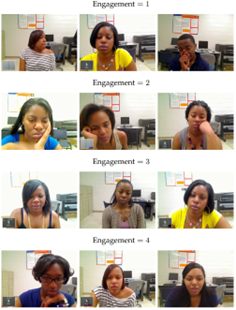
\includegraphics[width=0.4\linewidth]{images/2.png}
        \caption{Esempio campioni dal dataset dello studio}
    \end{center}
\end{figure}


Lo studio si concentra sull’effettuare una stima dell’engagement degli studenti. 

È stato inizialmente sviluppato un metodo per rilevare automaticamente l’engagement, si è poi indagato su quali segnali siano utilizzati nel riconoscimento automatico effettuato dal computer per poi individuare quali strumenti vengano adoperati dagli insegnanti per risolvere il medesimo task.

Infine si è investigato sulla correlazione effettiva fra i risultati di queste analisi e la qualità delle performance degli studenti.

\subsection{Facial coding as a mean to enable continuous monitoring of student’s behaviour in e-Learning [6]:}

Il paper si focalizza sul tracciamento continuo degli studenti, sia per quanto riguarda una vera e propria identificazione degli stessi attraverso il riconoscimento facciale, sia per calcolarne il livello di attenzione ed eventualmente stimarne le emozioni provate durante i corsi MOOCs (Massive Open Online Courses).

Per dirigere l’analisi del livello di attenzione, si è ricorso all’uso della libreria esterna Dlib, la quale consente di creare una mappatura delle caratteristiche facciali dello/a studente; per giunta, la piattaforma include anche un gaze tracker che lascia prevedere la direzione dello sguardo degli studenti durante lo svolgimento del corso.

Questi tre aspetti vengono successivamente congiunti al fine di creare un applicativo web per l’apprendimento attraverso il quale, alla fine di ogni lezione, è possibile visionare in quale percentuale della durata del corso le persone hanno adempito alle metriche sopracitate.

\begin{figure}
    \begin{center}    
        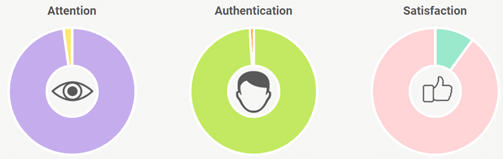
\includegraphics[width=1\linewidth]{images/3.png}
        \caption{Esempio output del programma}
    \end{center}
\end{figure}
 
\subsection{Prediction and Localization of student engagement in the wild [7]:}

Questo studio, a differenza di altri, ha come premessa l’utilizzo delle immagini raccolte in ambienti non controllati per la creazione del modello che andrà successivamente ad effettuare la predizione per i nuovi campioni.

Per ambienti controllati, si intende setup di acquisizione dei video e delle immagini grazie ai quali non è possibile riscontrare problemi, quali scarsa illuminazione, occlusione ambientale, etc…

Per attuare ciò, sono stati sottoposti ad analisi molti studi precedentemente effettuati, per convenire al raccoglimento di campioni attraverso la visione, da parte dei soggetti, di video educazionali, categorizzando poi i vari video ed immagini ottenute in una scala, con valore da 0 a 3:
\begin{itemize}
    \item 0 \textrightarrow per niente interessato (il soggetto non sembra interessato e guarda spesso al di fuori dello schermo)
    \item 1 \textrightarrow poco interesse (il soggetto apre a malapena gli occhi, si muove in modo irrequieto sulla sedia)
    \item 2 \textrightarrow interessato/a al contenuto (sembra che al soggetto il contenuto riprodotto risulti interessante ed esso interagisce con questo)
    \item 3 \textrightarrow altamente interessato/a (il soggetto ha “gli occhi attaccati allo schermo” e risulta concentrato/a)
\end{itemize}


Hanno poi sfruttato un framework che esegue il riconoscimento dell’engagement e della localizzazione degli studenti.
\begin{itemize}
    \item Inizialmente vengono identificate la faccia e dei punti di riferimento all’interno di queste in ognuno dei frame analizzati 
    \item Procedendo, i video vengono suddivisi in segmenti più piccoli e le feature vengono estratte, “effettuando una media” dei risultati di ognuno dei frame.
    \item Si passa poi alla sequenza di frame successiva per effettuare la stessa analisi.
    \item Una volta raccolti tutti i dati, questi vengono elaborati per calcolarne l’engagement e la localizzazione attraverso la deep MIL network, impiegando la media e la top-k pooling per calcolarne la regressione.
\end{itemize}


\begin{figure}
    \begin{center}    
        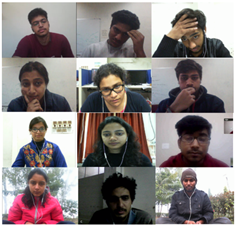
\includegraphics[width=0.6\linewidth]{images/4.png}
        \caption{Esempio di campioni dal loro dataset}
    \end{center}
\end{figure}


\section{Studi sul riconoscimento delle emozioni FACS per scelta del modello da utilizzare}
Essendo l’ammontare di studi che trattano l’analisi delle emozioni FACS maggiore rispetto a quelle che cercano di creare sistemi di riconoscimento automatico per gli stati d’animo, che possono direttamente aiutare a identificare i problemi nell’apprendimento delle conoscenze, ho ritenuto corretto studiare e scegliere fra i modelli da loro proposti per l’elaborazione delle informazioni per il mio caso di studio.

Fra i vari studi analizzati, per arrivare ad una conclusione circa la scelta del modello, quello risultato più utile è stato [2]: 

in questo studio vengono utilizzate le CNN (Convolutional Neural Networks); queste estraggono le feature facciali dalle immagini che successivamente vengono date in input a classificatori standard per eseguire la catalogazione di queste emozioni.

Nello studio ci si è valso dei dataset FER 2013 e RAF DB per l’analisi delle emozioni FACS (felicità, tristezza, sorpresa, paura, disgusto, rabbia, stato neutrale), si è poi ricorso a diversi metodi per l’analisi dei dati estratti, e i risultati di ognuno di questi sono stati confrontati fra di loro:

Nello specifico i metodi utilizzati sono:

\begin{itemize}
    \item STN (Spatial Transformer Networks): reti neurali utilizzate per effettuare la trasformazione geometrica degli input, ovvero per eseguire operazioni di rotazione, traslazione e scaling sui dati di input. Queste reti sono in grado di apprendere in maniera automatica tali trasformazioni e di applicarle direttamente ai dati di input.
    \begin{figure}
        \begin{center}    
            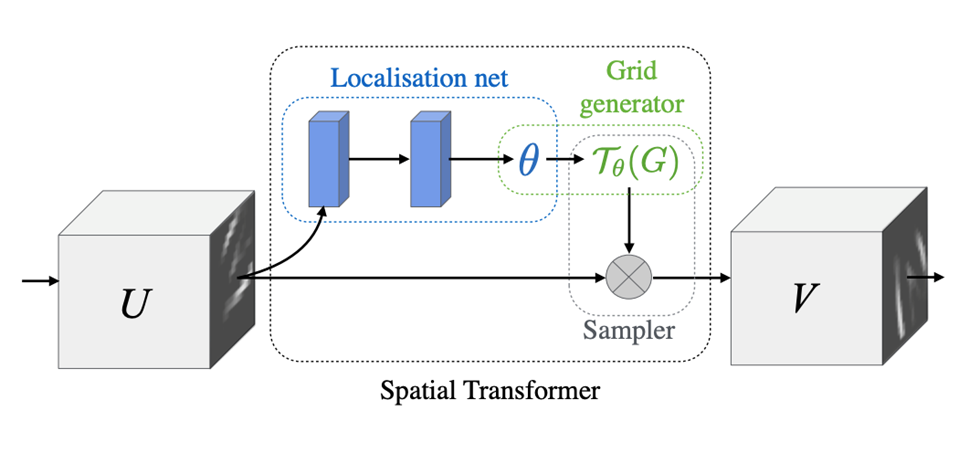
\includegraphics[width=0.9\linewidth]{images/5.png}
            \caption{implementazione STN}
        \end{center}
    \end{figure}
    \item SE (Squeeze and Excitation Networks): tecnica di rete neurale che si concentra sullo sfruttare la correlazione tra i canali delle feature map, al fine di migliorare la loro rappresentazione. Sostanzialmente, le reti SE "estraggono" (squeeze) i dati di input in un singolo vettore, calcolano l'importanza di ogni canale e "stimolano" (excite) i più rilevanti, migliorando così la qualità delle feature map.
    \begin{figure}
        \begin{center}    
            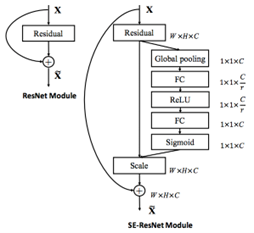
\includegraphics[width=0.5\linewidth]{images/6.png}
            \caption{implementazione SE}
        \end{center}
    \end{figure}
    \item BAM (Bottleneck Attention Module): modulo di attenzione che utilizza una tecnica di "bottleneck" per ridurre il numero di feature map da elaborare, rendendo il processo più efficiente. In particolare, il BAM sfrutta un'operazione di pooling per creare una rappresentazione ridotta dei dati di input, che viene poi sfruttata per calcolare l'attivazione di ogni canale delle feature map originali.
    \begin{figure}
        \begin{center}    
            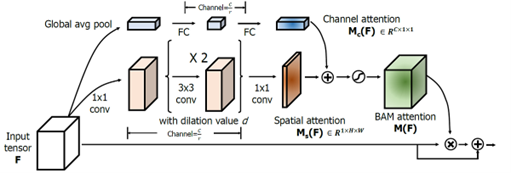
\includegraphics[width=0.9\linewidth]{images/7.png}
            \caption{implementazione BAM}
        \end{center}
    \end{figure}
    \item CBAM (Convolutional Bottleneck Attention Module): è una versione migliorata del BAM che utilizza sia l'attenzione spaziale che quella di canale. In pratica, il CBAM esegue prima un'operazione di attenzione spaziale per calcolare l'importanza delle diverse regioni dell'immagine, e successivamente utilizza un'operazione di attenzione di canale per calcolare la rilevanza dei diversi canali nelle feature map. Questo rende il CBAM particolarmente utile per il riconoscimento di oggetti in immagini complesse.   
    \begin{figure}
        \begin{center}    
            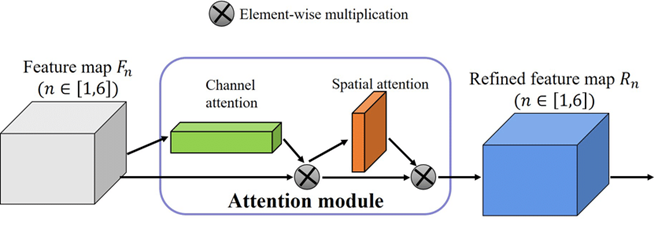
\includegraphics[width=0.9\linewidth]{images/8.png}
            \caption{implementazione CBAM}
        \end{center}
    \end{figure} 
\end{itemize}

Effettuando un confronto fra questi, il modello BAM è quello che offre una performance migliore sui due dataset, e a seguire l’STN.
Le emozioni che [2] si propone di valutare non sono esattamente quelle predisposte per lo studio di questa tesi, ma le valutazioni estratte da questo  si possono ritenere un buon metodo di valutazione del modello da scegliere.


    \begin{figure}
        \begin{center}    
            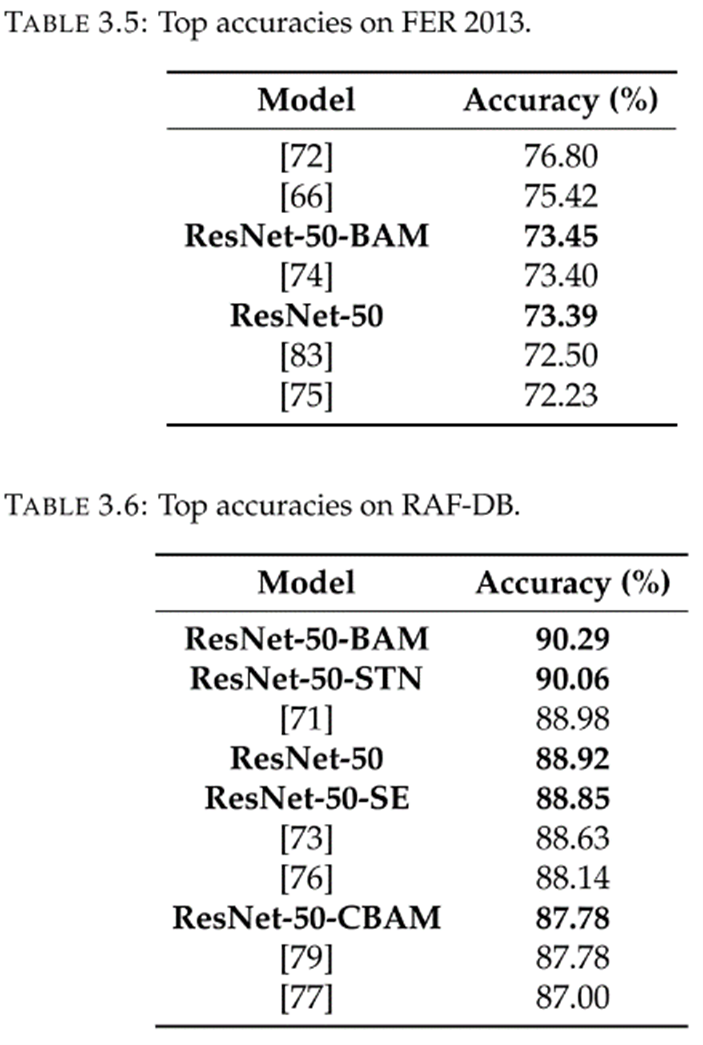
\includegraphics[width=0.4\linewidth]{images/9.png}
            \caption{Confronto fra i modelli}
        \end{center}
    \end{figure}
